\chapter{The Dragon and the Beasts: The Victory of the Lamb (12:1--14:20)}\index{dragon}\index{Lamb, the}

Revelation 12 and 13 draw extensively upon the visions and imagery of Genesis and Daniel\index{Daniel}. If we overlook these Old Testament backgrounds, we may be tempted to interpret the visions according to our own imaginations and, in doing so, misunderstand their meaning. This chapter therefore invites readers to return to the Old Testament, explore the roots of these symbols, and discover the spiritual conflict Revelation portrays: the struggle between the powers opposed to God and His unfolding plan of redemption\index{redemption}.

Why, then, can God's people overcome\index{overcomers} the devil? Revelation 12:11 gives us the answer: they overcome him “by the blood of the Lamb\index{Lamb, the!blood of} and by the word of their testimony.” The Christian struggle involves more than the people and circumstances we can see; beneath the visible world lies a deeper spiritual battle. The church does not conquer the dragon\index{dragon} through its own strength. Its victory rests upon the blood of the Lamb and upon a faithful testimony that endures even in suffering.

Chapter 14 then lifts our gaze to heaven, where angels proclaim the eternal gospel\index{eternal gospel} and call the inhabitants of the earth to fear God and give Him glory\index{glory}. Why, even at this late hour, does God still send His angels to proclaim the gospel?

What can endure beyond this fleeting earthly life?

The answer is found in receiving God's abundant grace\index{grace} and faithfully following Christ. To labor for the Lord, bear witness to Him, and nurture disciples while we remain on earth is itself a blessing. As Revelation 14:13 declares, those who die in the Lord are blessed, for their deeds follow them. These words remind us that our labor for Christ is never in vain. Even when believers endure suffering, they can persevere in faith, sustained by the hope that their faithful service will not be forgotten.

To help readers grasp the background and meaning of these visions without losing sight of the central theme—the victory of the Lamb\index{Lamb, the}—I have prepared the following table. It provides an overview of the visions, their Old Testament foundations, and their symbolic significance.

{
\small
\renewcommand{\arraystretch}{1}
\setlength{\tabcolsep}{4pt}

\begin{longtable}{
  >{\raggedright\arraybackslash}p{0.21\textwidth}
  >{\raggedright\arraybackslash}p{0.25\textwidth}
  >{\raggedright\arraybackslash}p{0.39\textwidth}
}
\caption{Old Testament background to the visions of Revelation 12--13}
\label{tab:rev12-13-ot-background} \\
\hline
Vision in Revelation &
Old Testament Background &
Symbolic Significance\\
\hline
\endfirsthead

\multicolumn{3}{l}{\small\itshape Table~\thetable\ (continued)} \\
\hline
Vision in Revelation &
Old Testament Background &
Symbolic Significance\\
\hline
\endhead

\hline
\endfoot

\hline
\endlastfoot

The woman &
Gen. 37:9--11; Isa. 54:1--8; 66:7--9 &
Israel and God's covenant people \\

The dragon &
Gen. 3:1--15 &
The ancient serpent, Satan, and the powers opposed to God \\

Seven heads and ten horns &
Dan. 7:7--8, 24 &
The imperial powers that oppose God \\

The male child &
Ps. 2:7--9 &
Jesus Christ, the Messianic King \\

The iron scepter &
Ps. 2:9 &
The Messiah's rule over the nations \\

1,260 days, forty-two months, and three and a half years &
Dan. 7:25; 12:7 &
A limited period of suffering; the powers opposed to God remain under His restraint \\

The war in heaven &
Dan. 10:13, 20--21; 12:1 &
The spiritual conflict taking place in the heavenly realm \\

The beast from the sea &
Dan. 7:2--8 &
Imperial power opposed to God and His people \\

The ten horns &
Dan. 7:7, 24 &
Political power exercised by kings \\

The beast from the earth &
Dan. 7; Rev. 13:11 &
A power that resembles the Lamb outwardly but speaks with the dragon's authority, deceiving the world \\

The mark on the forehead and hand &
Ex. 13:9, 16; Deut. 6:8; 11:18 &
God's people are to keep His words upon their hands and foreheads; the beast's mark signifies allegiance and belonging to the beast \\

666 &
&
The power opposed to God and its radical incompleteness \\

\end{longtable}
}

\begin{ReaderQuestion}
Almost every symbol in Table~\ref{tab:rev12-13-ot-background} has roots in the Old Testament. How might reading Revelation alongside the rest of Scripture protect us from speculation or misunderstanding?
\end{ReaderQuestion}

\section{The Woman: Israel}\index{Israel}

\begin{ScriptureBox2}{Circle how the woman and the dragon are each described. What is the dragon waiting to do?}

\item[12:1] A great sign appeared in heaven: a woman clothed with the sun, with the moon under her feet and a crown of twelve stars on her head.

\item[12:2] She was pregnant and cried out in pain as she was about to give birth.

\item[12:3] Then another sign appeared in heaven: an enormous red dragon with seven heads and ten horns and seven crowns on its heads.

\item[12:4] Its tail swept a third of the stars out of the sky and flung them to the earth. The dragon stood in front of the woman who was about to give birth, so that it might devour her child the moment he was born.

\end{ScriptureBox2}

\begin{figure}[htbp]
    \centering
    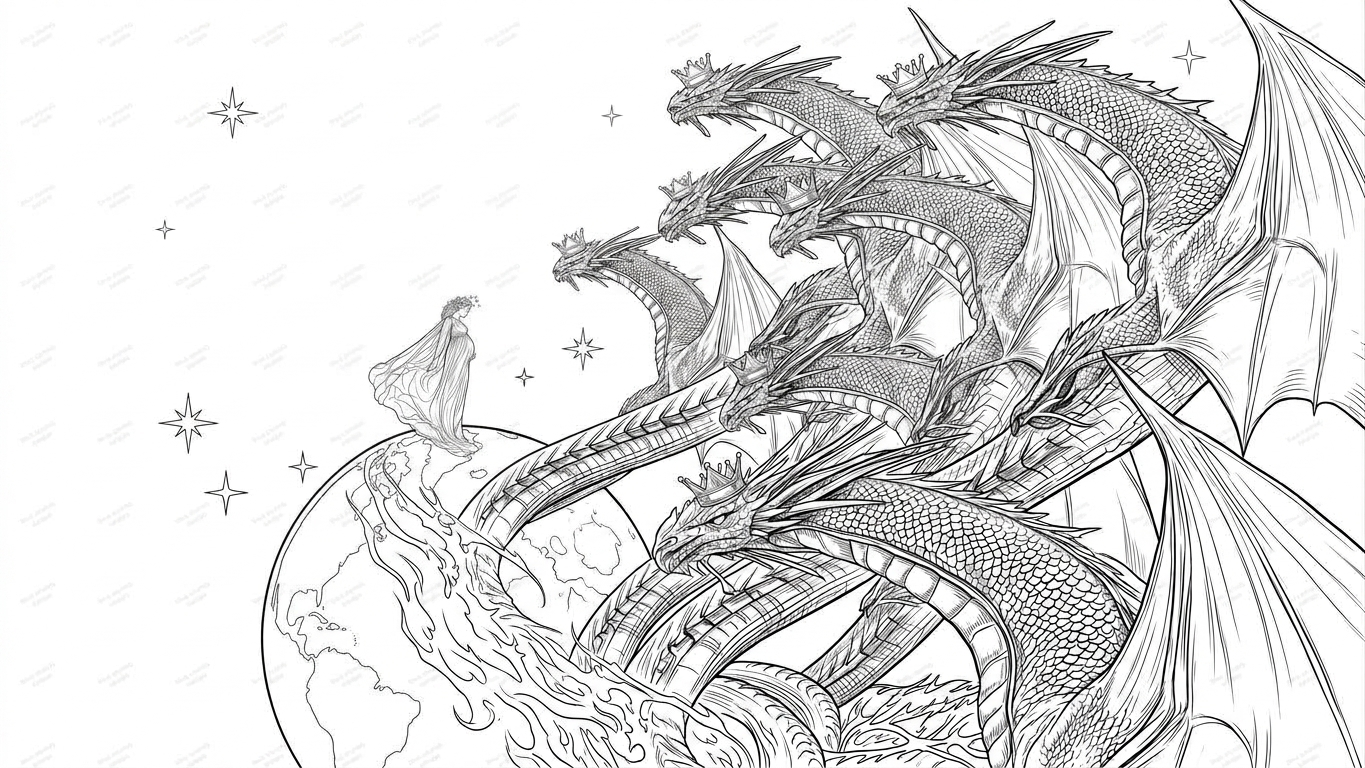
\includegraphics[
    width=1\textwidth,
    trim=0 0 0 0,
    clip]{images/woman_and_dragon2.jpg}
\end{figure}

The woman is clothed with the sun, has the moon beneath her feet, and wears a crown of twelve stars. Readers familiar with Scripture may immediately recall Joseph's dream in Genesis 37:9--11. In that dream, the sun, the moon, and eleven stars represent Jacob, Rachel, and Joseph's eleven brothers. Together with Joseph himself, the twelve stars also evoke the twelve tribes\index{twelve tribes of Israel} of Israel\index{Israel}.

Isaiah, too, repeatedly portrays God's people or Zion as a woman, using this image to describe the relationship between God and His people (Isa. 26:17--18; 49:14--23; 54:1--8; 66:7--9). Isaiah 66:7--9 is particularly significant, describing a woman who gives birth before her labor begins.

Taken together, these Old Testament images suggest that the woman represents Israel and, more broadly, God's covenant people.\footnote{G. K. Beale, \textit{The Book of Revelation: A Commentary on the Greek Text} (Grand Rapids, MI: Eerdmans, 1999), 625.}

Because the woman gives birth to the male child\index{male child}, who is the Messiah\index{Messiah}, Jesus Christ, some interpreters understand her to represent Mary, the mother of Jesus. Yet the imagery of the sun, moon, and twelve stars points more naturally to Israel understood in the broader sense of God's covenant people.

\section{The Male Child: Jesus Christ}\index{male child}

\begin{ScriptureBox2}{What will the male child do, and where is he taken?}

\item[12:5] \textit{She gave birth to a son, a male child, who “will rule all the nations with an iron scepter.” And her child was snatched up to God and to his throne.}

\end{ScriptureBox2}

This verse directly echoes Psalm 2:7--9, which declares, “You are my son; today I have become your father,” and speaks of the king ruling the nations with an iron scepter. The male child\index{male child} is therefore the Messianic King, Jesus Christ.

The vision moves swiftly from the child's birth to the dragon\index{dragon}'s attempt to destroy him, then immediately to the outcome: the child is caught up to God's throne\index{throne of God}. His earthly birth, death, resurrection, and ascension are not narrated in detail. Instead, the vision compresses the great events of redemption into a few striking images.

John is not attempting to recount Jesus' earthly life. His focus is elsewhere: the dragon\index{dragon} cannot destroy the Messiah\index{Messiah} whom God has appointed as King.\footnote{This is an example of a typological or redemptive-historical reading. A typological reading considers how people, events, and institutions in the Old Testament anticipate Christ. A redemptive-historical reading places a passage within the unfolding story of God's plan of salvation, tracing its place in the movement from creation and the Fall to redemption and final fulfillment. The emphasis is on the progression of God's saving work.}


\begin{ScriptureBox2}{Underline the three ways God's people triumph over the accuser in 12:11. How is the woman protected from the dragon, and against whom does the dragon then wage war?}

\item[12:6] The woman fled into the wilderness to a place prepared for her by God, where she might be taken care of for 1,260 days.

\item[12:7] Then war broke out in heaven. Michael and his angels fought against the dragon, and the dragon and his angels fought back.

\item[12:8] But he was not strong enough, and they lost their place in heaven.

\item[12:9] The great dragon was hurled down---that ancient serpent called the devil, or Satan, who leads the whole world astray. He was hurled to the earth, and his angels with him.

\item[12:10] Then I heard a loud voice in heaven say:\\
\hspace*{1em}``Now have come the salvation and the power\\
\hspace*{2em}and the kingdom of our God,\\
\hspace*{2em}and the authority of his Messiah.\\
\hspace*{1em}For the accuser of our brothers and sisters,\\
\hspace*{2em}who accuses them before our God day and night,\\
\hspace*{2em}has been hurled down.

\item[12:11] \hspace*{1em}They triumphed over him\\
\hspace*{2em}by the blood of the Lamb\\
\hspace*{2em}and by the word of their testimony;\\
\hspace*{1em}they did not love their lives so much\\
\hspace*{2em}as to shrink from death.

\item[12:12] \hspace*{1em}Therefore rejoice, you heavens\\
\hspace*{2em}and you who dwell in them!\\
\hspace*{1em}But woe to the earth and the sea,\\
\hspace*{2em}because the devil has gone down to you!\\
\hspace*{1em}He is filled with fury,\\
\hspace*{2em}because he knows that his time is short.''

\item[12:13] When the dragon saw that he had been hurled to the earth, he pursued the woman who had given birth to the male child.

\item[12:14] The woman was given the two wings of a great eagle, so that she might fly to the place prepared for her in the wilderness, where she would be taken care of for a time, times and half a time, out of the serpent's reach.

\item[12:15] Then from his mouth the serpent spewed water like a river, to overtake the woman and sweep her away with the torrent.

\item[12:16] But the earth helped the woman by opening its mouth and swallowing the river that the dragon had spewed out of his mouth.

\item[12:17] Then the dragon was enraged at the woman and went off to wage war against the rest of her offspring---those who keep God's commands and hold fast their testimony about Jesus.

\end{ScriptureBox2}

\begin{figure}[htbp]
    \centering
    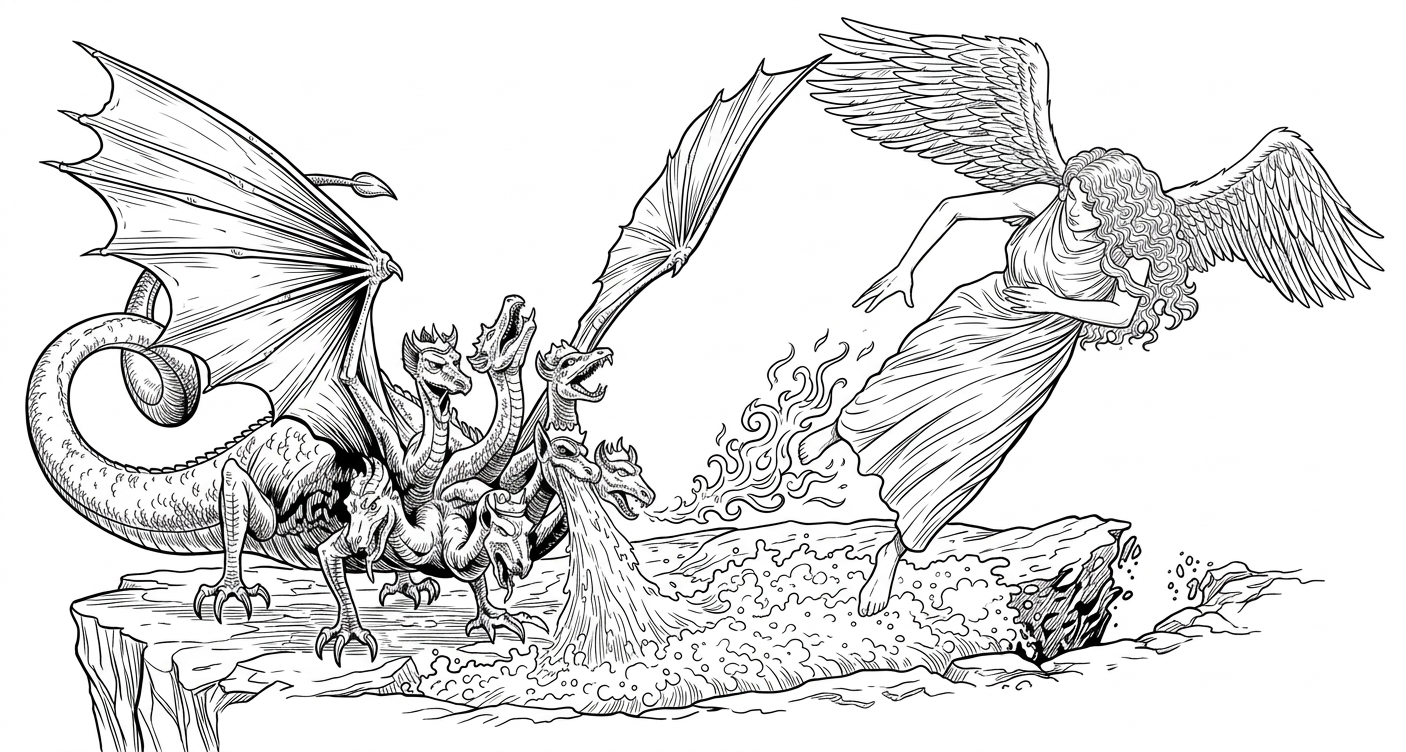
\includegraphics[
    width=1\textwidth,
    trim=0 0 0 0,
    clip]{images/woman_fly_away.jpg}
\end{figure}

The period of 1,260 days\index{1,260 days} is equivalent to three and a half years, using a 360-day year (1,260 divided by 360 equals 3.5). Daniel\index{Daniel} also refers to this period in several visions. Attempts to identify it too rigidly with a specific three-and-a-half-year period in a particular generation, however, can become strained and distract from the vision's central message.


\begin{ReaderQuestion}
The dragon's fury grows fiercer, yet its time is limited by God, and the woman is sustained in the wilderness. When you face a season of trial that seems to intensify rather than ease, how does knowing that God sets its limits and sustains you through it change the way you endure?
\end{ReaderQuestion}



\section{The Beast from the Sea: Imperial Power Opposed to God}\index{beast!from the sea}

\begin{ScriptureBox2}{Circle the animals the beast resembles. Who gives the beast its power, and how long may it exercise its authority?}

\item[13:1] The dragon stood on the shore of the sea. And I saw a beast coming out of the sea. It had ten horns and seven heads, with ten crowns on its horns, and on each head a blasphemous name.
% NIV footnote for 13:1 (omitted; add as \footnote if wanted):
%   ``The dragon'' --- Some later manuscripts And I
% NOTE: some translations number ``The dragon stood on the shore of the sea''
%   as 12:18; the NIV places it at 13:1.

\item[13:2] The beast I saw resembled a leopard, but had feet like those of a bear and a mouth like that of a lion. The dragon gave the beast his power and his throne and great authority.

\item[13:3] One of the heads of the beast seemed to have had a fatal wound, but the fatal wound had been healed. The whole world was filled with wonder and followed the beast.

\item[13:4] People worshiped the dragon because he had given authority to the beast, and they also worshiped the beast and asked, ``Who is like the beast? Who can wage war against it?''

\item[13:5] The beast was given a mouth to utter proud words and blasphemies and to exercise its authority for forty-two months.

\item[13:6] It opened its mouth to blaspheme God, and to slander his name and his dwelling place and those who live in heaven.

\item[13:7] It was given power to wage war against God's holy people and to conquer them. And it was given authority over every tribe, people, language and nation.

\item[13:8] All inhabitants of the earth will worship the beast---all whose names have not been written in the Lamb's book of life, the Lamb who was slain from the creation of the world.
% NIV footnote for 13:8 (omitted; add as \footnote if wanted):
%   ``from the creation of the world'' --- Or written from the creation of
%   the world in the book of life belonging to the Lamb who was slain

\item[13:9] Whoever has ears, let them hear.

\item[13:10] \hspace*{1em}``If anyone is to go into captivity,\\
\hspace*{2em}into captivity they will go.\\
\hspace*{1em}If anyone is to be killed with the sword,\\
\hspace*{2em}with the sword they will be killed.''\\
This calls for patient endurance and faithfulness on the part of God's people.
% NIV footnotes for 13:10 (omitted; add as \footnote if wanted):
%   ``is to be killed'' --- Some manuscripts anyone kills
%   ``they will be killed'' --- Jer. 15:2
% CHECK NIV: all footnote wording in this passage quoted from memory;
%   verify against Bible Gateway.

\end{ScriptureBox2}

The beast\index{beast} represents earthly imperial power opposed to God. We see the foundation for this interpretation in Daniel\index{Daniel}. Daniel 7 describes four beasts rising from the sea and explains that they represent four kings who will arise on the earth. Daniel 8 then presents the vision of a ram and a goat, foretelling the rise of Medo-Persia and Greece, the emergence of a Greek king, and the subsequent division of the Greek empire.\footnote{The king is commonly identified as Alexander the Great (Dan. 8:21), who conquered Persia in the fourth century BC, roughly two centuries after the time traditionally associated with Daniel.}

These visions establish an important pattern: beasts represent earthly rulers and imperial powers.

In Revelation, after the dragon\index{dragon} is cast down, it takes its stand on the shore of the sea. What does it do next? It brings into view the beast from the sea\index{beast!from the sea} and the beast from the earth\index{beast!from the earth}. What, then, does the sea beast represent? Its features point directly back to Daniel 7.

In Revelation, the sea symbolizes the peoples and nations of the world. Revelation 17:15 explicitly interprets the waters as peoples, multitudes, nations, and languages. The beast rising from the sea therefore represents earthly power emerging from among the nations and standing in opposition to God and His people.

Table \ref{tab:rev13-daniel7} compares the vision in Revelation 13 with its Old Testament background in Daniel 7.

{
\renewcommand{\arraystretch}{1}
\small
\begin{longtable}{>{\raggedright\arraybackslash}p{3cm}
                  >{\raggedright\arraybackslash}p{3.5cm}
                  >{\raggedright\arraybackslash}p{2.7cm}}
\caption{The beast of Revelation 13 and the beasts of Daniel 7}
\label{tab:rev13-daniel7} \\
\hline
Revelation 13 &
Daniel 7 &
Significance \\
\hline
\endfirsthead

\multicolumn{3}{l}{\small\itshape Table~\thetable\ (continued)} \\
\hline
Revelation 13 &
Daniel 7 &
Significance \\
\hline
\endhead

\hline
\endfoot

\hline
\endlastfoot

1: The beast rises from the sea &
2--3: Four beasts rise from the sea &
Empires among the nations \\

2: The beast has a lion's mouth &
4: The first beast resembles a lion &
Lion imagery \\

2: The beast has feet like a bear's &
5: The second beast resembles a bear &
Bear imagery \\

2: The beast resembles a leopard &
6: The third beast resembles a leopard &
Leopard imagery \\

1: The beast possesses terrifying power &
7: The fourth beast is exceedingly terrifying &
Power surpassing that of earlier empires \\

1: The beast has ten horns &
7: The fourth beast has ten horns &
Imperial power \\

6: The beast speaks blasphemies &
8: The little horn speaks boastfully &
Usurping God's authority \\

7: The beast wages war against the saints &
21: The little horn wages war against the holy people &
Persecution of God's people \\

7: The beast overcomes the saints &
21: The little horn overpowers them &
A temporary victory \\

The Lamb ultimately judges the beast &
22: The Ancient of Days takes His place in judgment &
Final judgment \\

5: Forty-two months &
25: A time, times, and half a time &
A limited period of persecution \\

7: The beast is permitted to wage war against the saints &
25: The holy people are handed over to the beast &
God permits but limits its power \\

The beast faces God's judgment &
26--27: The beast's dominion is finally taken away &
The beast's ultimate defeat \\

\end{longtable}
}

\begin{ReaderQuestion}
In Table~\ref{tab:rev13-daniel7}, the beast of Revelation 13 combines features of all four beasts in Daniel 7: the lion, the bear, the leopard, and the ten horns. It even ``overcomes the saints,'' yet the table ends with its dominion taken away. What powers in today's world seem impressive or frightening to you, and how does this table help you see them in light of God's final judgment?
\end{ReaderQuestion}

One of the most striking features of this vision is that the dragon\index{dragon} gives its authority to the sea beast. One of the beast's heads appears to have suffered a fatal wound, yet the wound is healed, and the whole world marvels and follows the beast. Here we see a counterfeit of Christ's death and resurrection.

The true Christ suffered death, rose again, and was exalted in glory. The beast, by contrast, appears to have died but recovers, and then receives the worship\index{worship} of the world. It imitates the pattern of Christ's victory, offering a deceptive spectacle in place of the true work of redemption.

\begin{figure}[htbp]
    \centering
    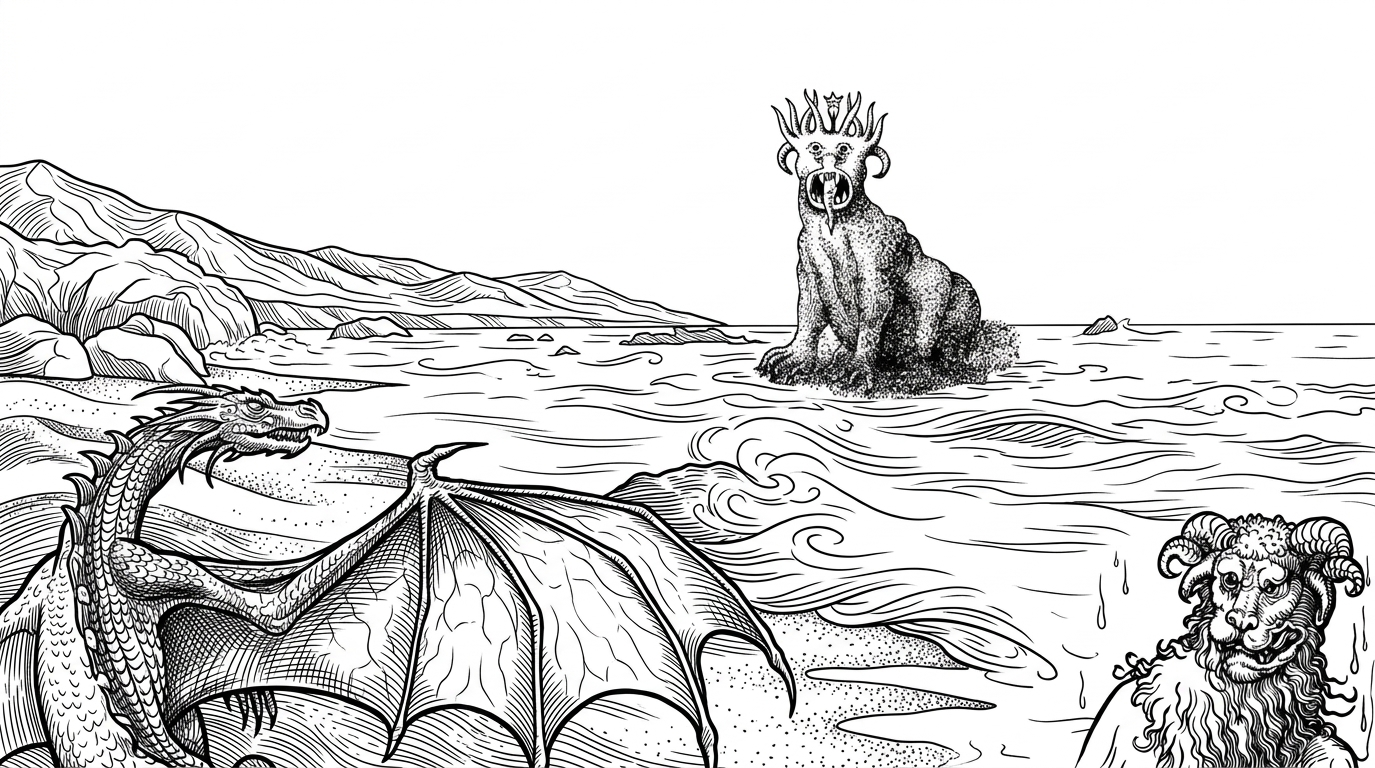
\includegraphics[
    width=1\textwidth,
    trim=0 0 0 0,
    clip]{images/dragon_and_breast.jpg}
\end{figure}

\section{The Beast from the Earth: The False Prophet}\index{beast!from the earth}\index{false prophet}

\begin{ScriptureBox2}{What does the second beast look like, and how does it speak? Underline everything it makes the inhabitants of the earth do.}

\item[13:11] Then I saw a second beast, coming out of the earth. It had two horns like a lamb, but it spoke like a dragon.

\item[13:12] It exercised all the authority of the first beast on its behalf, and made the earth and its inhabitants worship the first beast, whose fatal wound had been healed.

\item[13:13] And it performed great signs, even causing fire to come down from heaven to the earth in full view of the people.

\item[13:14] Because of the signs it was given power to perform on behalf of the first beast, it deceived the inhabitants of the earth. It ordered them to set up an image in honor of the beast who was wounded by the sword and yet lived.

\item[13:15] The second beast was given power to give breath to the image of the first beast, so that the image could speak and cause all who refused to worship the image to be killed.

\end{ScriptureBox2}

Now we turn to the beast from the earth\index{beast!from the earth}. It has two horns like a lamb, yet it speaks like a dragon\index{dragon}. Its appearance suggests innocence and even a resemblance to the Lamb, but its voice betrays its true allegiance. This is a deceptive religious power. Later, Revelation 16:13, 19:20, and 20:10 identify it as the false prophet\index{false prophet}.

\begin{ReaderQuestion}
The beast from the earth looks like a lamb but speaks like a dragon. How does this image help us discern teachings that appear godly on the surface but are actually deceptive?
\end{ReaderQuestion}

The beast from the earth\index{beast!from the earth} is therefore not simply another political empire. It operates under the authority of the first beast, performing signs, deceiving people, promoting the worship of the beast\index{beast}, and leading the inhabitants of the earth to accept its mark.

Together, the dragon\index{dragon}, the beast from the sea\index{beast!from the sea}, and the beast from the earth\index{beast!from the earth} form a counterfeit trinity. The dragon imitates God, the sea beast imitates the Lamb, and the false prophet\index{false prophet} imitates the work of the Holy Spirit\index{Holy Spirit}. Their apparent unity is a dark parody of the true God: a counterfeit kingdom that seeks to claim the worship, allegiance, and trust that belong to God alone.

\begin{ReaderQuestion}
How do the dragon, the beast from the sea, and the beast from the earth work together to imitate God's authority and oppose Him? What does this teach us about spiritual warfare?
\end{ReaderQuestion}

\section{The Number of Man: 666}\index{666}

\begin{ScriptureBox2}{Who is forced to receive the mark, and where is it placed? What can people not do without it?}

\item[13:16] It also forced all people, great and small, rich and poor, free and slave, to receive a mark on their right hands or on their foreheads,

\item[13:17] so that they could not buy or sell unless they had the mark, which is the name of the beast or the number of its name.

\item[13:18] This calls for wisdom. Let the person who has insight calculate the number of the beast, for it is the number of a man. That number is 666.
% NIV footnote for 13:18 (omitted; add as \footnote if wanted):
%   ``the number of a man'' --- Or is humanity's number
% CHECK NIV: footnote wording quoted from memory; verify against Bible Gateway.

\end{ScriptureBox2}

Those who receive the beast\index{beast}'s mark are permitted to buy and sell. Those who refuse it, by contrast, face exclusion from ordinary economic life. God's servants who will not accept the mark may find themselves unable to participate in the marketplace and forced to rely on barter or other means of survival. Their refusal to worship the beast comes at a considerable cost.

Yet they remain faithful to the truth: only the Lamb who was slain\index{Lamb, the!slain} is worthy of worship. Through the blood of the Lamb\index{Lamb, the!blood of} and the faithful testimony they maintain, His people overcome\index{overcomers} even amid the beast's persecution\index{persecution}.

Why is the number 666\index{666} rather than 777? It is unwise to treat 666 simply as a secret code that can be used to identify some particular person, object, or technology. In Scripture, the number seven is often associated with completeness or fullness. The triple six, by contrast, can be understood as a picture of radical incompleteness: a repeated falling short of the fullness represented by seven. The contrast is striking. God's perfection stands in opposition to the beast's arrogant self-exaltation, which can never attain the fullness that belongs to God.

Some have associated the beast's mark with modern technology, barcodes, microchips, identity cards, or cashless payment systems. Such associations may arise naturally when modern readers reflect on the text, but they should not be treated as direct predictions of particular future technologies. The passage's central concern is allegiance and worship: whom people worship, to whom they give their loyalty, and how that loyalty can expose them to social and economic persecution\index{persecution}.

\begin{ReaderQuestion}
How does the mark of the beast contrast with the faithfulness of God's people? When faith conflicts with economic interests or social pressure, how can we remain steadfast?
\end{ReaderQuestion}

\section{The Lamb and His People}\index{Lamb, the}

The vision of the dragon\index{dragon}, the sea beast, and the earth beast presents a disturbing counterfeit of the divine order. Yet chapter 14 redirects our gaze to the Lamb.

John sees the Lamb standing on Mount Zion, accompanied by 144,000\index{144,000} people. The names of the Lamb and His Father are written on their foreheads, marking them as belonging to God rather than to the beast\index{beast}. They follow the Lamb wherever He goes, remaining faithful to God's commandments and to their testimony about Jesus even through times of tribulation.

The counterfeit trinity of chapter 13 stands in sharp contrast to the Lamb and His people in chapter 14. The beast demands worship, but the Lamb's people worship Him. The world may use power, fear, and material advantage to pressure people into compromise, but God knows those who belong to Him. The mark of the beast\index{beast!mark of} may appear to determine who can participate in earthly society; the name of the Lamb reveals who truly belongs to the kingdom that will endure.

Then three angels announce the coming judgment\index{judgment}. The first proclaims the eternal gospel\index{eternal gospel}, calling all nations to fear God and give Him glory. The second announces the fall of Babylon\index{Babylon}. The third warns that those who worship the beast will face God's judgment. Finally, two harvest\index{harvest} visions bring us to the end of the age: the grain is ripe, the grapes are fully mature, and God's judgment will surely come.

Amid these solemn warnings, however, God gives His people a precious word of comfort:

“Blessed are the dead who die in the Lord.”

Though they have labored on earth and some have even laid down their lives for Christ, their labor has not been in vain. They will rest from their toil, and their deeds will follow them. The world may forget their faithfulness, but the Lord does not. The Lamb who calls them to endure is the same Lamb who will receive them into His presence.

\begin{ScriptureBox2}{What is written on the foreheads of the 144,000? Underline every phrase that describes them in 14:4--5.}

\item[14:1] Then I looked, and there before me was the Lamb, standing on Mount Zion, and with him 144,000 who had his name and his Father's name written on their foreheads.

\item[14:2] And I heard a sound from heaven like the roar of rushing waters and like a loud peal of thunder. The sound I heard was like that of harpists playing their harps.

\item[14:3] And they sang a new song before the throne and before the four living creatures and the elders. No one could learn the song except the 144,000 who had been redeemed from the earth.

\item[14:4] These are those who did not defile themselves with women, for they remained virgins. They follow the Lamb wherever he goes. They were purchased from among mankind and offered as firstfruits to God and the Lamb.

\item[14:5] No lie was found in their mouths; they are blameless.

\end{ScriptureBox2}

%\begin{figure}[htbp]
%    \centering
%    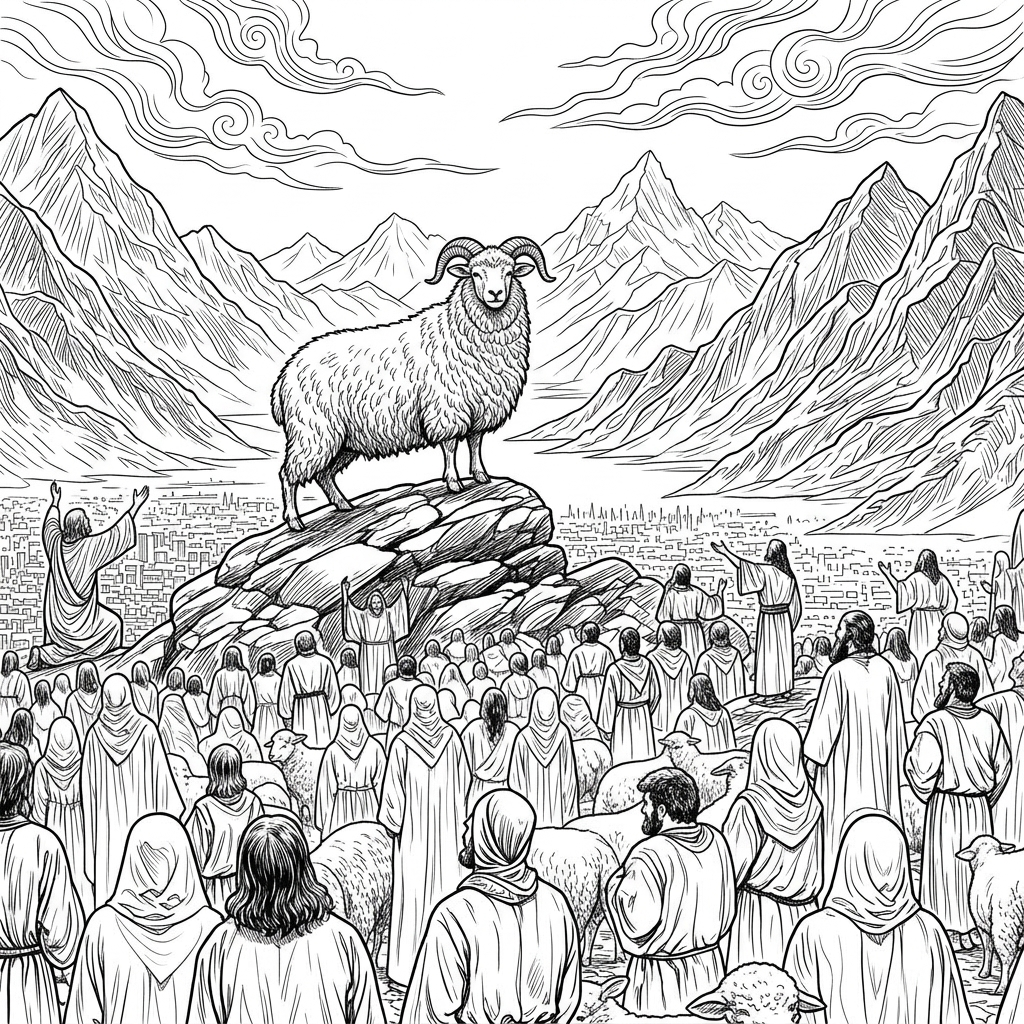
\includegraphics[
%    width=1\textwidth,
%    trim=0 0 0 0,
%    clip]{images/lamb_14400.jpg}
%\end{figure}

These people are described as having been “purchased from among mankind and offered as firstfruits to God and the Lamb.” They are redeemed by Jesus and belong to Him. The declaration that no lie is found in their mouths and that they are blameless does not mean that they have achieved sinless perfection through their own efforts. Rather, they stand before the Lamb as those who belong to Him, cleansed and made acceptable through His redemptive work.

They are also described as those who “did not defile themselves with women, for they remained virgins.” Some interpret this description literally, understanding them to be unmarried men who have abstained from sexual relations. Yet the Old Testament frequently uses the imagery of marriage and sexual unfaithfulness to portray faithfulness or unfaithfulness to God. In this context, the language also conveys the idea of undivided loyalty to the Lamb. Wherever He goes, they follow.

\begin{ReaderQuestion}
What does it mean to you personally to follow the Lamb wherever He goes (Rev. 14:4)?
\end{ReaderQuestion}

Their song is unlike any other. It is a song born of a journey through redemption, a song that can be learned only by those who have walked the path themselves and remained steadfast through trial. Its melody rises from lives purchased by the Lamb and kept faithful to Him. No one else can learn this new song, because its praise springs from an experience of grace and perseverance known only to those who have followed the Lamb through suffering.

\section{The Angels Proclaim the Eternal Gospel}\index{eternal gospel}

\begin{ScriptureBox2}{Underline what each of the three angels proclaims. Who are called blessed in 14:13, and why?}

\item[14:6] Then I saw another angel flying in midair, and he had the eternal gospel to proclaim to those who live on the earth---to every nation, tribe, language and people.

\item[14:7] He said in a loud voice, ``Fear God and give him glory, because the hour of his judgment has come. Worship him who made the heavens, the earth, the sea and the springs of water.''

\item[14:8] A second angel followed and said, ``\,`Fallen! Fallen is Babylon the Great,' which made all the nations drink the maddening wine of her adulteries.''
% NIV footnote for 14:8 (omitted; add as \footnote if wanted):
%   ``Fallen is Babylon the Great'' --- Isaiah 21:9
% CHECK NIV: footnote reference quoted from memory; verify against Bible Gateway.

\item[14:9] A third angel followed them and said in a loud voice: ``If anyone worships the beast and its image and receives its mark on their forehead or on their hand,

\item[14:10] they, too, will drink the wine of God's fury, which has been poured full strength into the cup of his wrath. They will be tormented with burning sulfur in the presence of the holy angels and of the Lamb.

\item[14:11] And the smoke of their torment will rise for ever and ever. There will be no rest day or night for those who worship the beast and its image, or for anyone who receives the mark of its name.''

\item[14:12] This calls for patient endurance on the part of the people of God who keep his commands and remain faithful to Jesus.

\item[14:13] Then I heard a voice from heaven say, ``Write this: Blessed are the dead who die in the Lord from now on.''\\
``Yes,'' says the Spirit, ``they will rest from their labor, for their deeds will follow them.''

\end{ScriptureBox2}

\begin{figure}[h]
    \centering
    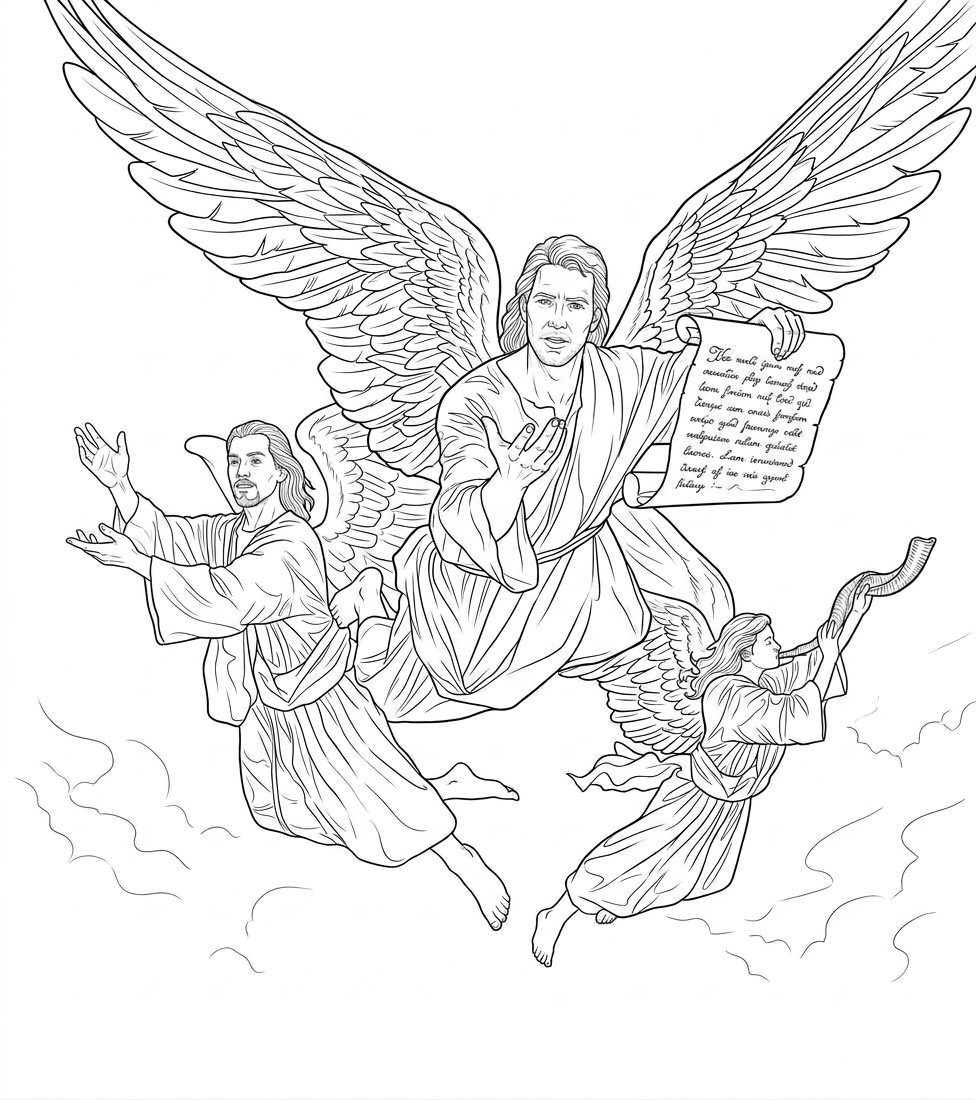
\includegraphics[
    width=0.8\textwidth,
    trim=0 0 0 0,
    clip]{images/eternal_gospel.jpg}
\end{figure}

Even at this late hour, the gospel is still proclaimed to the inhabitants of the earth. What does this eternal gospel\index{eternal gospel} declare? It calls people to fear God, give Him glory, and worship the One who made the heavens, the earth, the sea, and the springs of water.

Our very existence is a gift of the Creator\index{Creator}. As creatures who have received the grace of life, we are called to respond by worshiping God and giving Him the glory that belongs to Him. The eternal gospel\index{eternal gospel} therefore summons all people to recognize their Creator and turn to Him in reverence and worship.

\begin{ReaderQuestion}
What does the first angel's proclamation of the “eternal gospel” include (Rev. 14:6--7)? Why are fearing God, giving Him glory, and worshiping the Creator integral to the message of the gospel?
\end{ReaderQuestion}

The next two angels announce God's righteous judgment. Those who rebel against their Creator\index{Creator} reject not only the grace of being created but also the redeeming blood of Jesus Christ. They give their allegiance to the beast\index{beast}, receive its mark, and persecute\index{persecution} the saints. God's judgment upon those who persist in such rebellion is therefore not arbitrary. It is the just response of the holy God to the rejection of His rule and the oppression of His people.

Yet for those who persevere in faith, and for those who die in the Lord, there is a blessed promise. They truly rest from their toil, and the fruit of their labor for Christ follows them. What a profound comfort this is to those who have spent their lives serving the Lord, often without recognition, and sometimes at great personal cost. Their work may appear small in the eyes of the world, but it is not forgotten in heaven.

\section{The Two Visions of the Harvest}\index{harvest}

\begin{ScriptureBox2}{Compare the two harvests. Who swings the first sickle, what is gathered in the second, and where is it thrown?}

\item[14:14] I looked, and there before me was a white cloud, and seated on the cloud was one like a son of man with a crown of gold on his head and a sharp sickle in his hand.
% NIV footnote for 14:14 (omitted; add as \footnote if wanted):
%   ``son of man'' --- See Daniel 7:13.

\item[14:15] Then another angel came out of the temple and called in a loud voice to him who was sitting on the cloud, ``Take your sickle and reap, because the time to reap has come, for the harvest of the earth is ripe.''

\item[14:16] So he who was seated on the cloud swung his sickle over the earth, and the earth was harvested.

\item[14:17] Another angel came out of the temple in heaven, and he too had a sharp sickle.

\item[14:18] Still another angel, who had charge of the fire, came from the altar and called in a loud voice to him who had the sharp sickle, ``Take your sharp sickle and gather the clusters of grapes from the earth's vine, because its grapes are ripe.''

\item[14:19] The angel swung his sickle on the earth, gathered its grapes and threw them into the great winepress of God's wrath.

\item[14:20] They were trampled in the winepress outside the city, and blood flowed out of the press, rising as high as the horses' bridles for a distance of 1,600 stadia.
% NIV footnote for 14:20 (omitted; add as \footnote if wanted):
%   ``1,600 stadia'' --- That is, about 180 miles or about 300 kilometers
% CHECK NIV: footnote wording quoted from memory; verify against Bible Gateway.

\end{ScriptureBox2}

As discussed in earlier chapters, the figure described here as “one like a son of man\index{Son of Man}” is Jesus Christ. The harvest\index{harvest} is ripe, and He holds a sharp sickle in His hand, ready to reap the earth.

In John 4:35, Jesus speaks of the harvest\index{harvest} in words familiar to those who work the land. He tells His disciples to lift their eyes and look at the fields, for they are ripe for harvest. Imagine a field of golden grain, its heavy heads bending in the light, while workers move through it with sharp sickles. What a joyful sight it is when the harvest has come!

Yet harvest\index{harvest} is also an image of judgment. The grain and the weeds are separated: the grain is gathered into the barn, while the weeds are burned. In Matthew 13:24--30, Jesus uses a parable drawn from ordinary agricultural life to teach this truth. The farmer does not attempt to separate the wheat from the weeds while the plants are still young. Both are allowed to grow together until the harvest, when their true nature becomes clear and they can be separated.\footnote{Matthew 13:24--30 recounts Jesus' parable of the wheat and the weeds. An enemy sows weeds among the wheat while the household sleeps. When the plants grow, the servants ask whether they should pull out the weeds. The owner refuses, lest they uproot the wheat as well. Both are to grow together until the harvest, when the weeds will be gathered and burned and the wheat brought into the barn. Insert the licensed NIV text here if the full passage is to be quoted.}

The connection between harvest\index{harvest} and judgment is made explicit in Joel 3:13, which calls for the sickle to be put in because the harvest is ripe, and for the winepress\index{winepress} to be trodden because the winepress is full and the vats overflow with the wickedness of the nations.

In Revelation, an angel swings his sickle over the earth and gathers the grapes, throwing them into the great winepress\index{winepress} of God's wrath\index{wrath of God}. The time of judgment has arrived. The image is terrible in its force: the wickedness of the earth has ripened, and the judgment of God can no longer be deferred.

As grapes are crushed in the winepress until the vats overflow, so the vision portrays the overwhelming severity of divine judgment. The blood rises as high as the horses' bridles and extends for a distance of 1,600 stadia, a scene of judgment rendered in stark and unforgettable imagery.

\begin{ReaderQuestion}
Revelation 14 shows two harvests: the grain gathered by the Son of Man and the grapes thrown into the winepress of God's wrath. Since the final harvest has not yet come, how should God's patience today shape the way you respond to Him, and the way you speak to others about Him?
\end{ReaderQuestion}

\begin{figure}[htbp]
    \centering
    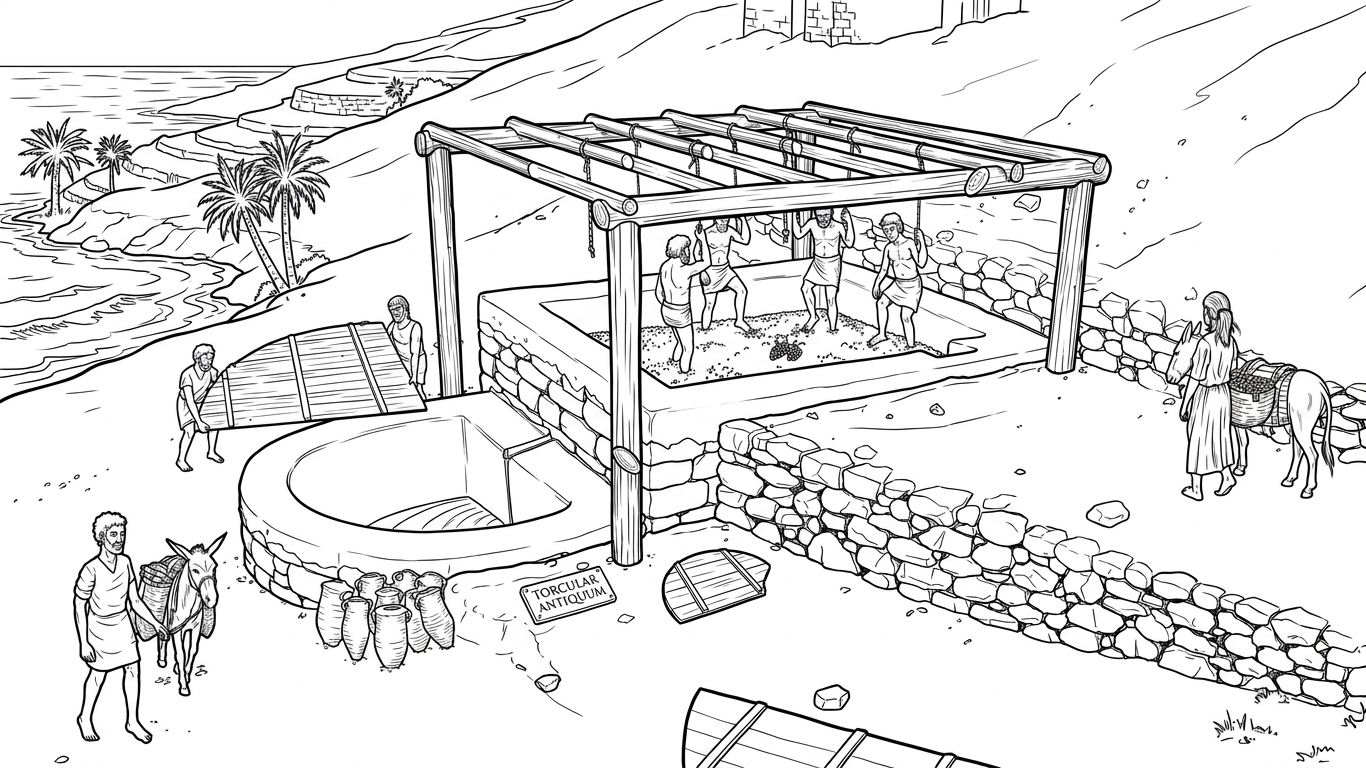
\includegraphics[
    width=1\textwidth,
    trim=0 0 0 0,
    clip]{images/wine_pressing.jpg}
\end{figure}
